%Notes by Harsh Mistry 
%CS 444
%based on Template from : https://www.cs.cmu.edu/~ggordon/10725-F12/template.tex

\documentclass{article}
\setlength{\oddsidemargin}{0.25 in}
\setlength{\evensidemargin}{-0.25 in}
\setlength{\topmargin}{-0.6 in}
\setlength{\textwidth}{6.5 in}
\setlength{\textheight}{8.5 in}
\setlength{\headsep}{0.75 in}
\setlength{\parindent}{0 in}
\setlength{\parskip}{0.1 in}
\usepackage{amsfonts,graphicx, amssymb}
\usepackage[fleqn]{amsmath}
\usepackage{fixltx2e}
\usepackage{color}
\usepackage{tcolorbox}
\usepackage{lipsum}
\usepackage{listings}
\graphicspath{ {./images/} }
\usepackage{scrextend}
\tcbuselibrary{skins,breakable}
\usetikzlibrary{shadings,shadows}
\newcounter{lecnum}
\renewcommand{\thepage}{\thelecnum-\arabic{page}}
\renewcommand{\thesection}{\thelecnum.\arabic{section}}
\renewcommand{\theequation}{\thelecnum.\arabic{equation}}
\renewcommand{\thefigure}{\thelecnum.\arabic{figure}}
\renewcommand{\thetable}{\thelecnum.\arabic{table}}
\newcommand{\lecture}[4]{
   \pagestyle{myheadings}
   \thispagestyle{plain}
   \newpage
   \setcounter{lecnum}{#1}
   \setcounter{page}{1}
   
   
%Info Box 
   \begin{center}
   \framebox{
      \vbox{\vspace{2mm}
    \hbox to 6.28in { {\bf CS 444 - Compiler Construction 
	\hfill Winter 2020} }
       \vspace{4mm}
       \hbox to 6.28in { {\Large \hfill Lecture #1: #2  \hfill} }
       \vspace{2mm}
       \hbox to 6.28in { {\it Lecturer: #3 \hfill Notes By: #4} }
      \vspace{2mm}}
   }
   \end{center}
   
   \markboth{Lecture #1: #2}{Lecture #1: #2}



 
}

\renewcommand{\cite}[1]{[#1]}
\def\beginrefs{\begin{list}%
        {[\arabic{equation}]}{\usecounter{equation}
         \setlength{\leftmargin}{2.0truecm}\setlength{\labelsep}{0.4truecm}%
         \setlength{\labelwidth}{1.6truecm}}}
\def\endrefs{\end{list}}
\def\bibentry#1{\item[\hbox{[#1]}]}

\newcommand{\fig}[3]{
			\vspace{#2}
			\begin{center}
			Figure \thelecnum.#1:~#3
			\end{center}
	}
	
\newcommand{\pipe}{\(\mid\)}
\newcommand{\ctr}{\(\wedge\)}

\newtheorem{theorem}{Theorem}[lecnum]
\newtheorem{lemma}[theorem]{Lemma}
\newtheorem{ex}[theorem]{Example}
\newtheorem{proposition}[theorem]{Proposition}
\newtheorem{claim}[theorem]{Claim}
\newtheorem{corollary}[theorem]{Corollary}
\newtheorem{definition}[theorem]{Definition}
\newenvironment{proof}{{\bf Proof:}}{\hfill\rule{2mm}{2mm}}
\newcommand\E{\mathbb{E}}

%color definitions :
\definecolor{darkred}{rgb}{0.55, 0.0, 0.0}
\definecolor{lightcoral}{rgb}{0.94, 0.5, 0.5}
\definecolor{tomato}{rgb}{1.0, 0.39, 0.28}
\definecolor{lightgray}{rgb}{.9,.9,.9}
\definecolor{darkgray}{rgb}{.4,.4,.4}
\definecolor{purple}{rgb}{0.65, 0.12, 0.82}
\definecolor{lightgreen}{rgb}{0.56, 0.93, 0.56}
\definecolor{darkgreen}{rgb}{0.0, 0.2, 0.13}
\definecolor{limegreen}{rgb}{0.2, 0.8, 0.2}
\definecolor{lightblue}{rgb}{0.68, 0.85, 0.9}
\definecolor{darkblue}{rgb}{0.0, 0.0, 0.55}


%Environments
\newenvironment{exblock}[1]{%
    \tcolorbox[beamer,%
    noparskip,breakable,
    colback=lightgreen,colframe=darkgreen,%
    colbacklower=limegreen!75!lightgreen,%
    title=#1]}%
    {\endtcolorbox}

\newenvironment{ablock}[1]{%
    \tcolorbox[beamer,%
    noparskip,breakable,
    colback=lightcoral,colframe=darkred,%
    colbacklower=tomato!75!lightcoral,%
    title=#1]}%
    {\endtcolorbox}

\newenvironment{cblock}[1]{%
    \tcolorbox[beamer,%
    noparskip,breakable,
    colback=lightblue,colframe=darkblue,%
    colbacklower=darkblue!75!lightblue,%
    title=#1]}%
    {\endtcolorbox}


%Languages
\lstdefinelanguage{JavaScript}{
  keywords={typeof, new, true, false, catch, function, return, null, catch, switch, var, if, in,  fi, while, do, else, case, break},
  keywordstyle=\color{blue}\bfseries,
  ndkeywords={class, export, boolean, throw, implements, import, this},
  ndkeywordstyle=\color{darkgray}\bfseries,
  identifierstyle=\color{black},
  sensitive=false,
  comment=[l]{//},
  morecomment=[s]{/*}{*/},
  commentstyle=\color{purple}\ttfamily,
  stringstyle=\color{red}\ttfamily,
  morestring=[b]',
  morestring=[b]"
}

%Listings
\lstset{
   language=JavaScript,
   backgroundcolor=\color{lightgray},
   extendedchars=true,
   basicstyle=\footnotesize\ttfamily,
   showstringspaces=false,
   showspaces=false,
   numbers=left,
   numberstyle=\footnotesize,
   numbersep=9pt,
   tabsize=2,
   breaklines=true,
   showtabs=false,
   captionpos=b
}


%Start of Document 
\begin{document}

\lecture{4}{January 15th, 2020}{Ond\u{r}ej Lhot\'{a}k}{Harsh Mistry}

\section{Analysis Continued}

\subsection{Parsing}
\begin{itemize}
\item The ultimate goal is to produce a tree data structure which represents the input
\item Regular expressions can express infinite languages, but not infinite levels of nesting.Therefore for parsing we use context-free languages  represented by a context-free grammar 
\end{itemize}

\begin{definition} Context Free Grammar (CFG) is a 4-tuple \(G = <N, T, R, S>\)
\begin{itemize}
\item \(T\) - Terminals 
\begin{itemize}
\item Words that make up the actual language
\end{itemize}
\item \(N\) - Non-Terminals
\begin{itemize}
\item Internal to the grammar
\end{itemize}
\item \(R\) - Production Rules

\item \(S\) - Start non-terminal
\end{itemize}
\end{definition}

\begin{itemize}
\item Notations in this course
\begin{itemize}
\item Terminals - \(a,b,c \in T\)
\item Non-terminals - \(A, B, C \in N\)
\item Start - \(S\)
\item Symbols - \(V = T \cup N\) \hspace{0.5cm} \(X, Y, Z \in T \cup N\) 
\item Strings of terminals \(T^*\) - \(w, x, y, z \in T^*\)
\item Strings of symbols \((T \cup N)^* \) - \(\alpha, \beta, \gamma, \delta \in (T \cup N)^*\)  
\item Production Rules - \( A \rightarrow \alpha\)
\end{itemize}
\end{itemize}

\begin{definition} "Directly Derives" 
\(BA \gamma \rightarrow P \alpha \gamma\) if \(A \rightarrow a \in E\)
\end{definition}

\begin{definition} "Derives" 
\(\alpha \rightarrow^* \beta\) if \(\alpha = \beta\) or \(\alpha \rightarrow \gamma\) and \(\gamma \rightarrow \beta\)
\end{definition}

\begin{definition} \(L(G) = \{ x \in T^* \mid S \rightarrow *x\}\)
\end{definition}

\begin{definition} \(\alpha\) is a \underline{sentential form} if \(S \rightarrow^* \alpha\)\\
\(L(G) = sentential-forms(G) \cap  T^* \)
\end{definition}
\begin{definition}  Recognition is \(x \in L(G)\) 
\end{definition}

\begin{itemize}
\item Parsing is finding a \underline{derivation} for \(x\)
\end{itemize}
\begin{exblock}{Example}
\textbf{Grammar}:
\begin{itemize}
\item \(A \rightarrow B g C\)
\item \(C \rightarrow ef\)
\item \(B \rightarrow ab\)
\end{itemize}
\textbf{Derivation:}
\begin{itemize}
\item Right Canonical : \(A \rightarrow B g C \rightarrow Bgef \rightarrow abgef\)
\item Left Canonical: \(A \rightarrow B g C \rightarrow abgC \rightarrow ef \)
\end{itemize}
\begin{center}
\begin{tikzpicture}
\node[draw] at (0,0) {A};
\draw (0.4,0) -- (3,-2.5);
\draw (-0.4,0) -- (-3,-2.5);
\draw (0,-0.4) -- (0,-2.5);

\node[draw] at (-3,-3) {B};
\node[draw] at (0,-3) {g};
\node[draw] at (3,-3) {C};

\draw (-3.4,-3) -- (-5,-4.5);
\draw (-2.6,-3) -- (-1,-4.5);
\draw (2.6,-3) -- (1,-4.5);
\draw (3.4,-3) -- (5,-4.5);

\node[draw] at (-5,-5) {a};
\node[draw] at (-1,-5) {b};
\node[draw] at (1,-5) {e};
\node[draw] at (5,-5) {f};
\end{tikzpicture}
\end{center}
\end{exblock}



\begin{definition}
A grammar is \underline{Ambiguous} if some input has more than 1 parse tree
\end{definition}
\newpage
\subsubsection{Top-Down Parsing}
\textbf{LL(k) LL(1)}
\begin{itemize}
\item Start with \(\alpha = S\) and input string \(x\)
\item Repeat till \(\alpha = x\)
\begin{itemize}
\item Replace some non-terminal \(A\) in \(\alpha\) with \(\beta\) where \(A \rightarrow B \in R\)
\end{itemize}
\end{itemize}

\begin{center}



\tikzset{every picture/.style={line width=0.75pt}} %set default line width to 0.75pt        

\begin{tikzpicture}[x=0.75pt,y=0.75pt,yscale=-1,xscale=1]
%uncomment if require: \path (0,300); %set diagram left start at 0, and has height of 300

%Shape: Triangle [id:dp21405750059505446] 
\draw   (171.25,112) -- (242.5,223) -- (100,223) -- cycle ;
%Straight Lines [id:da6290805767832155] 
\draw [color={rgb, 255:red, 74; green, 144; blue, 226 }  ,draw opacity=1 ]   (179.5,125) -- (120.5,223) ;


%Straight Lines [id:da6419620825733282] 
\draw [color={rgb, 255:red, 255; green, 0; blue, 0 }  ,draw opacity=1 ]   (163.5,179) -- (193.8,197.94) ;
\draw [shift={(195.5,199)}, rotate = 212.01] [color={rgb, 255:red, 255; green, 0; blue, 0 }  ,draw opacity=1 ][line width=0.75]    (10.93,-3.29) .. controls (6.95,-1.4) and (3.31,-0.3) .. (0,0) .. controls (3.31,0.3) and (6.95,1.4) .. (10.93,3.29)   ;


% Text Node
\draw (169,234) node   [align=left] {x};
% Text Node
\draw (171,96) node   [align=left] {S};


\end{tikzpicture}

\begin{ablock}{Note}
\(LL(k)\) grammars cannot generate left-associative trees
\end{ablock}


\end{center}

\subsubsection{Bottom-Up Parsing}
\textbf{LR(k) LR(1)}
\begin{itemize}
\item Start with \(\alpha = x\) 
\item Repeat till \(\alpha = S\)
\begin{itemize}
\item Replace some "handle" \(\beta\) in \(\alpha\) with A where \(A \rightarrow B \in R\)
\end{itemize}
\end{itemize}

\begin{center}


\tikzset{every picture/.style={line width=0.75pt}} %set default line width to 0.75pt        

\begin{tikzpicture}[x=0.75pt,y=0.75pt,yscale=-1,xscale=1]
%uncomment if require: \path (0,300); %set diagram left start at 0, and has height of 300

%Shape: Triangle [id:dp21405750059505446] 
\draw   (171.25,112) -- (242.5,223) -- (100,223) -- cycle ;
%Straight Lines [id:da6290805767832155] 
\draw [color={rgb, 255:red, 74; green, 144; blue, 226 }  ,draw opacity=1 ]   (128.5,182) -- (167.5,224) ;


%Straight Lines [id:da6419620825733282] 
\draw [color={rgb, 255:red, 255; green, 0; blue, 0 }  ,draw opacity=1 ]   (147.5,195) -- (190.92,161.23) ;
\draw [shift={(192.5,160)}, rotate = 502.13] [color={rgb, 255:red, 255; green, 0; blue, 0 }  ,draw opacity=1 ][line width=0.75]    (10.93,-3.29) .. controls (6.95,-1.4) and (3.31,-0.3) .. (0,0) .. controls (3.31,0.3) and (6.95,1.4) .. (10.93,3.29)   ;


% Text Node
\draw (169,234) node   [align=left] {x};
% Text Node
\draw (171,96) node   [align=left] {S};


\end{tikzpicture}

\end{center}

\begin{ablock}{Note}
\(LR(k)\) grammars can generate both left-associative and right-associative trees
\end{ablock}

\end{document}







